\documentclass[14pt]{article}
\usepackage[utf8]{inputenc}
\usepackage[T1]{fontenc}
\usepackage[norsk]{babel}
\usepackage{floatpag}				% Different pagestyles
\usepackage{amsmath}
\usepackage{array}	
\usepackage{booktabs}
\usepackage{amssymb}
\usepackage{graphicx}
\usepackage{epstopdf}
\usepackage{tabularx}
\usepackage{float}
\usepackage{caption}
\usepackage{subcaption}
\usepackage{parskip}
\usepackage{multirow}
\usepackage{listings}

\begin{document}
\title{Oblig 9}
\author{Magnus Isaksen}
\maketitle
\newpage 

\section*{Exercise 1}

\subsection*{a)}

Når vi skal finne multiplisiteten til en Einstein krystall med N oscillatorer og en total energi $E = q\Delta \epsilon$

q er antallet energipakker og representerer derfor den totale energien i systemet. 

N er antallet tilstander denne totale energien skal fordeles på. Altså hvordan energipakkene er fordelt i krystallen. 

Dermed for å finne multiplisiteten må man se på hvor mange mulige måter energipakkene kan fordeles i krystallen. 

Antall måter er $\Omega = \frac{(q+N-1)!}{(q+N-1-q)!(q!)} = \frac{(q+N-1)!}{q!(N-1)!}$ som da er det vi ville vise. 

\subsection*{b)}


Den idelle gasslov er $pV=TNk$ 

En adiabatisk prosess er når det ikke finnes noe varmeutveksling mellom omgivelsene og systemet. 

En isoterm prosess er når det er varmeutveksling mellom systemet og omgivelsene. 

I det isoterme tilfellet er temperaturen konstant siden systemet kan slippe ut energi til omgivelsene hvis det det blir for varmt eller ta inn energi hvis det er for kaldt. Men i den adiabatiske er vil temperaturen øke dersom volumet blir mindre og temperaturen øker, mens den vil minke hvis volumet blir større og trykket mindre. 

\newpage

\begin{figure}[ht!]
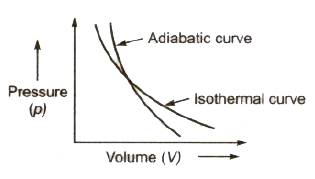
\includegraphics[width = \textwidth]{Graph_A.jpg}
\end{figure}

\subsection*{c)}

Endring i entropien i en ideell gass finner vi med. 

$\Delta S = \int_{T_1}^{T_2} \frac{C_V}{T} dT = 3Nk ln \frac{T_2}{T_1} $


\section*{Exercise 0.15}

\subsection*{a)}
Har $\varepsilon_i = S_i mB$ og partisjonsfunksjonen $Z = \sum_i exp{\beta \varepsilon_i } = \sum exp(\beta S_imB)$  med $\beta = \frac{1}{kT}$ dette gir for en spinn tilfellet med spinn muligheter opp og ned.

$Z = exp(-\beta \varepsilon ) + exp(\beta \varepsilon ) = 2cosh(\beta \varepsilon ) = 2cosh(\beta S_imB)$

\subsection*{b)}

For N spin tilstander 

$Z = \sum_{S_1} \sum_{S_2}...\sum_{S_N} exp(\frac{-\varepsilon (S_1 +S_2 ...S_N}{kT}) = Z_1^N$ 

Da alle har spinn opp og ned vil vi få samme partisjonsfunksjon for alle tilstanden og dermed har vi $Z = Z_1^N$ 

Da alle partikler er fiksert til spesielle punkt deler vi ikke med N! da de er adskillbare.

\subsection*{c)}

Helmholz fri energi finner vi med 

$F = -kT \ln (z_N) = -kT \ln (Z_1^N) = -kTN \ln (2 cosh(\frac{mB}{kT}) = -KTN ( \ln 2 + \ln (cosh(\frac{mB}{kT}))) $ 


\subsection*{d)}

Entropien er gitt som

$S = (\frac{\partial F}{\partial T})_{V,N}$

$S = - \frac{\partial }{\partial T} (-kTN(\ln 2 -\ln cosh(\frac{mB}{kT})))$

$S = kN(\ln 2 -\ln cosh(\frac{mB}{kT}) - \frac{mB}{kT}tanh(\frac{mB}{kT}))$

\subsection*{e)}

Gjennomsnitts spinnet finner vi ved 

$ \bar{S_i} = \sum S_i P(S_i) $

$ P(S_i) = \frac{1}{Z_i}\sum exp(-\varepsilon / kT)$

$ \bar{S_i} = \frac{1}{Z_1} (exp(-mB/kT) - exp(mB/kT))$ 

$\bar{S_i} = \frac{2sinh(\frac{mB}{kT})}{2cosh(\frac{mB}{kT})} = tanh(\frac{mB}{kT})$

\subsection*{f)}

Når B blir stor går gjennomsnittet mot 1. Da B feltet blir sterkt vil den rette spinnene i en retning.  

Når T blir stor går gjennomsnittet mot 0. Vil energien i partiklene føre til at B feltet ikke klarer å påvirke hvordan spinn partiklene har. 

\subsection*{g)}

Siden B og T er reelle tall vil B feltet påvirke hvordan spinnene retter seg. Dermed er sannsynlighetene alltid litt større mot 




\end{document}
